\documentclass{standalone}
\usepackage{tikz}
\usetikzlibrary{patterns, positioning}
\usepackage[sfdefault]{ClearSans} %% option 'sfdefault' activates Clear Sans as the default text font
\usepackage[T1]{fontenc}

\begin{document}
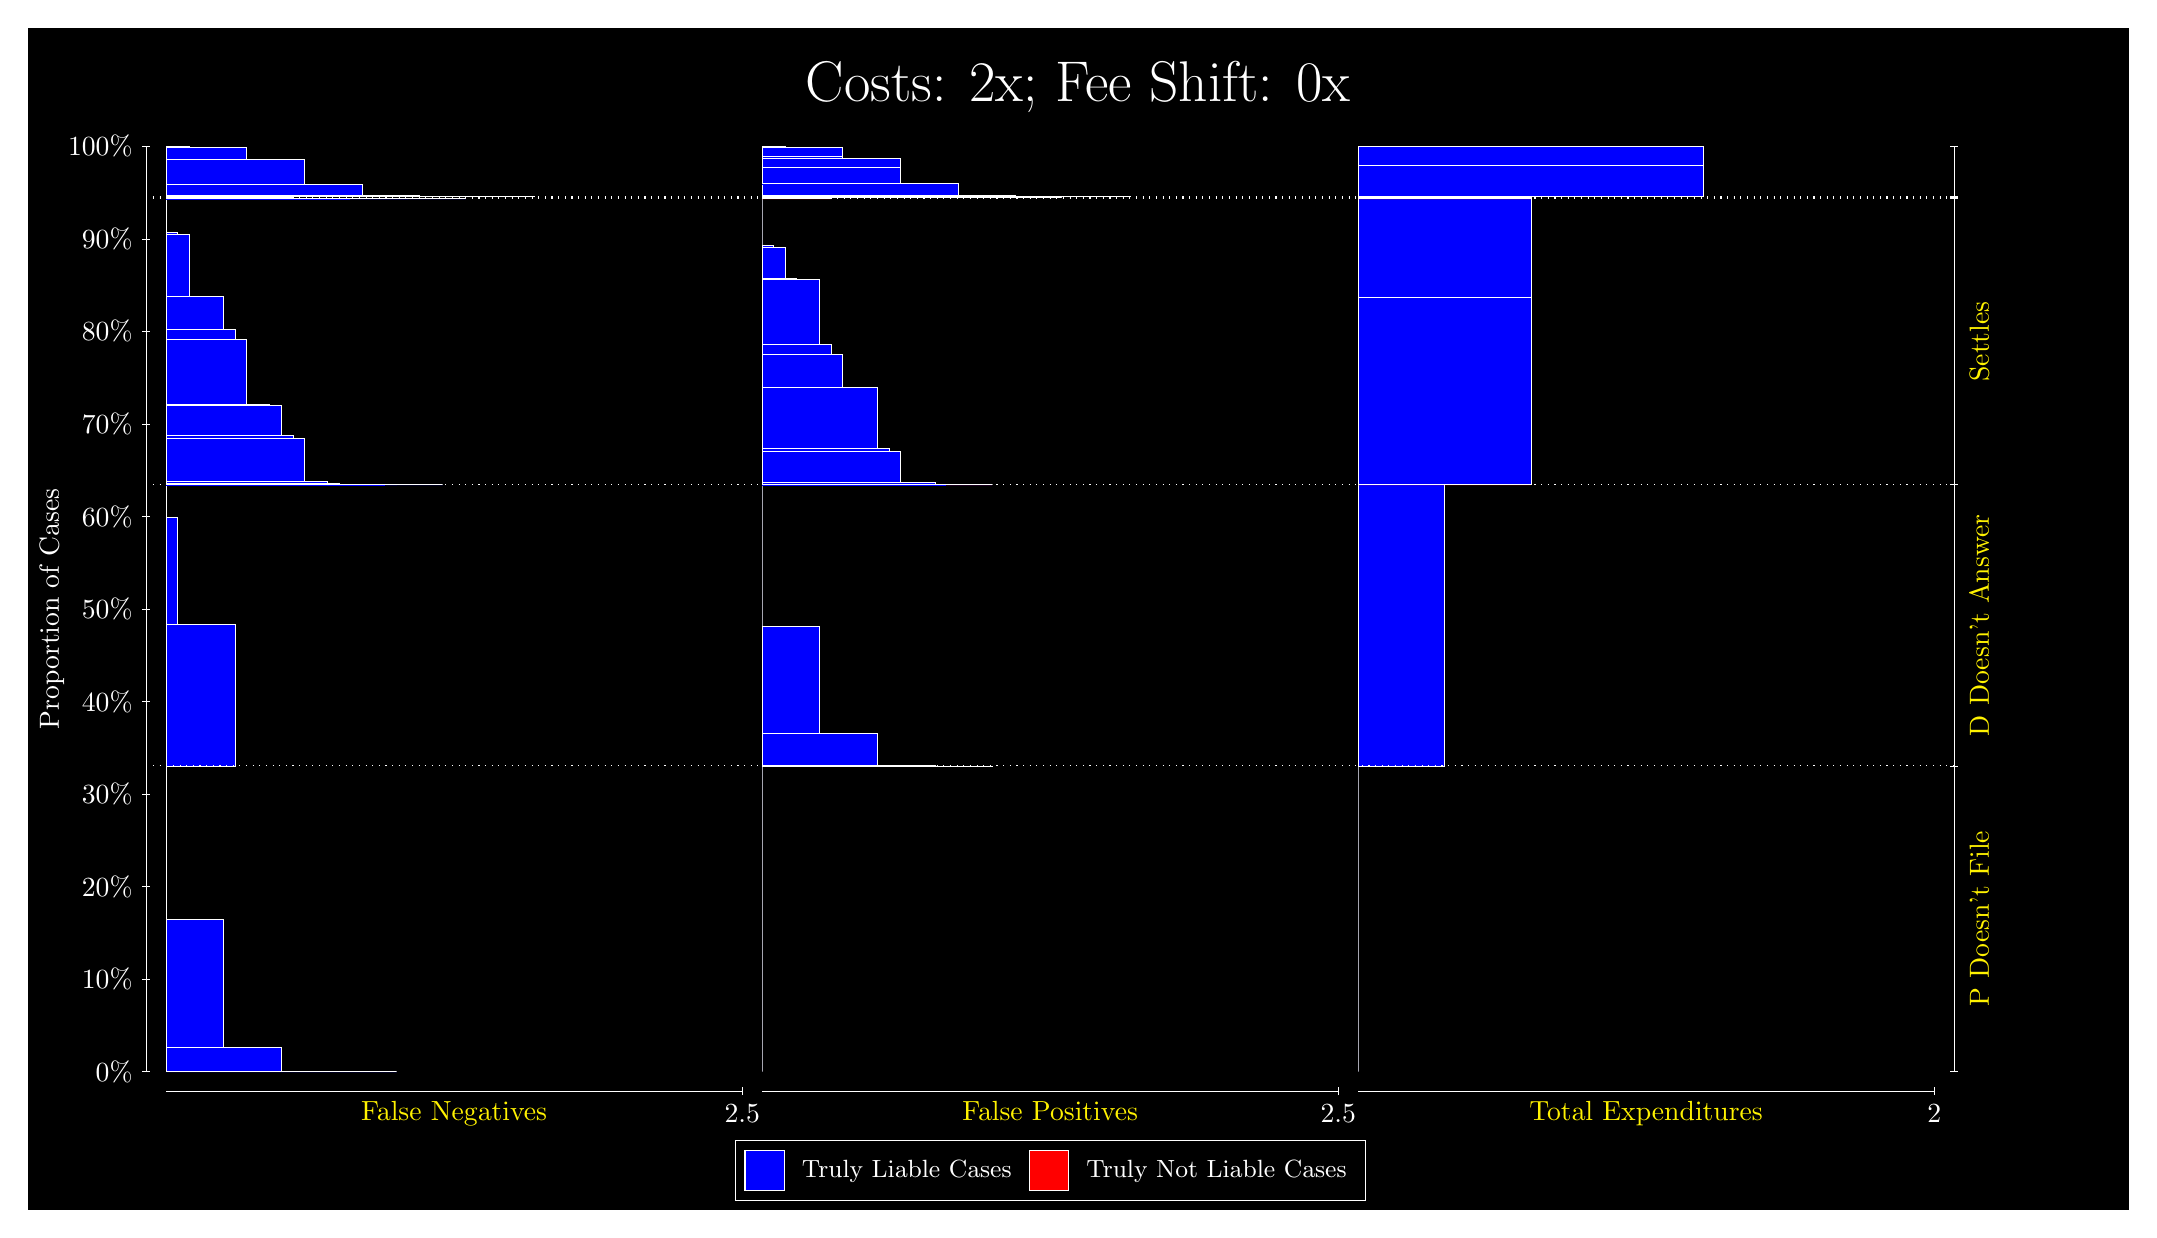
\begin{tikzpicture}
\draw[fill=black] (0,0) rectangle (26.667,15);
\draw[text=white] (0,13.5) rectangle (26.667,15) node[midway] {\huge Costs: 2x; Fee Shift: 0x};
\draw[white, very thin] (1.5,1.75) -- (1.5,13.5);
\node[rotate=90, text=white, anchor=center] at (0.3, 7.625) {Proportion of Cases};
\draw[white, very thin] (1.45,1.75) -- (1.55,1.75);
\node[text=white, anchor=east] at (1.45, 1.75) {0\%};
\draw[white, very thin] (1.45,2.925) -- (1.55,2.925);
\node[text=white, anchor=east] at (1.45, 2.925) {10\%};
\draw[white, very thin] (1.45,4.1) -- (1.55,4.1);
\node[text=white, anchor=east] at (1.45, 4.1) {20\%};
\draw[white, very thin] (1.45,5.275) -- (1.55,5.275);
\node[text=white, anchor=east] at (1.45, 5.275) {30\%};
\draw[white, very thin] (1.45,6.45) -- (1.55,6.45);
\node[text=white, anchor=east] at (1.45, 6.45) {40\%};
\draw[white, very thin] (1.45,7.625) -- (1.55,7.625);
\node[text=white, anchor=east] at (1.45, 7.625) {50\%};
\draw[white, very thin] (1.45,8.8) -- (1.55,8.8);
\node[text=white, anchor=east] at (1.45, 8.8) {60\%};
\draw[white, very thin] (1.45,9.975) -- (1.55,9.975);
\node[text=white, anchor=east] at (1.45, 9.975) {70\%};
\draw[white, very thin] (1.45,11.15) -- (1.55,11.15);
\node[text=white, anchor=east] at (1.45, 11.15) {80\%};
\draw[white, very thin] (1.45,12.325) -- (1.55,12.325);
\node[text=white, anchor=east] at (1.45, 12.325) {90\%};
\draw[white, very thin] (1.45,13.5) -- (1.55,13.5);
\node[text=white, anchor=east] at (1.45, 13.5) {100\%};

\draw[white, very thin] (24.457,1.75) -- (24.457,13.5);
\draw[white, very thin] (24.407,1.75) -- (24.507,1.75);
\node[anchor=west] at (24.407, 1.75) {};
\draw[white, very thin] (24.407,5.6315) -- (24.507,5.6315);
\node[anchor=west] at (24.407, 5.6315) {};
\draw[white, very thin] (24.407,9.2039) -- (24.507,9.2039);
\node[anchor=west] at (24.407, 9.2039) {};
\draw[white, very thin] (24.407,12.836) -- (24.507,12.836);
\node[anchor=west] at (24.407, 12.836) {};
\draw[white, very thin] (24.407,12.855) -- (24.507,12.855);
\node[anchor=west] at (24.407, 12.855) {};
\draw[white, very thin] (24.407,12.868) -- (24.507,12.868);
\node[anchor=west] at (24.407, 12.868) {};
\draw[white, very thin] (24.407,13.5) -- (24.507,13.5);
\node[anchor=west] at (24.407, 13.5) {};

\draw[white, very thin, fill=blue] (1.75,1.75) rectangle (4.6775,1.75);
\draw[white, very thin, fill=blue] (1.75,1.75) rectangle (3.9457,1.7526);
\draw[white, very thin, fill=blue] (1.75,1.7526) rectangle (3.2138,2.0581);
\draw[white, very thin, fill=blue] (1.75,2.0581) rectangle (2.4819,3.6826);
\draw[white, very thin, fill=red] (1.75,3.6826) rectangle (1.75,3.6826);
\draw[white, very thin, fill=blue] (1.75,3.6826) rectangle (1.75,5.6315);
\draw[white, very thin, fill=blue] (1.75,5.6315) rectangle (2.6283,7.4247);
\draw[white, very thin, fill=blue] (1.75,7.4247) rectangle (1.8964,8.7933);
\draw[white, very thin, fill=red] (1.75,8.7933) rectangle (1.75,8.7933);
\draw[white, very thin, fill=blue] (1.75,8.7933) rectangle (1.75,9.2039);
\draw[white, very thin, fill=blue] (1.75,9.2039) rectangle (5.2631,9.2039);
\draw[white, very thin, fill=blue] (1.75,9.2039) rectangle (4.6775,9.2039);
\draw[white, very thin, fill=blue] (1.75,9.2039) rectangle (4.5312,9.2043);
\draw[white, very thin, fill=blue] (1.75,9.2043) rectangle (4.092,9.2052);
\draw[white, very thin, fill=blue] (1.75,9.2052) rectangle (3.9457,9.22);
\draw[white, very thin, fill=blue] (1.75,9.22) rectangle (3.7993,9.2411);
\draw[white, very thin, fill=blue] (1.75,9.2411) rectangle (3.5065,9.7904);
\draw[white, very thin, fill=blue] (1.75,9.7904) rectangle (3.3602,9.8255);
\draw[white, very thin, fill=blue] (1.75,9.8255) rectangle (3.2138,10.214);
\draw[white, very thin, fill=blue] (1.75,10.214) rectangle (3.0674,10.23);
\draw[white, very thin, fill=blue] (1.75,10.23) rectangle (2.7746,11.05);
\draw[white, very thin, fill=blue] (1.75,11.05) rectangle (2.6283,11.181);
\draw[white, very thin, fill=blue] (1.75,11.181) rectangle (2.4819,11.597);
\draw[white, very thin, fill=blue] (1.75,11.597) rectangle (2.3355,11.597);
\draw[white, very thin, fill=blue] (1.75,11.597) rectangle (2.0428,12.381);
\draw[white, very thin, fill=blue] (1.75,12.381) rectangle (1.8964,12.414);
\draw[white, very thin, fill=red] (1.75,12.414) rectangle (1.75,12.414);
\draw[white, very thin, fill=blue] (1.75,12.414) rectangle (1.75,12.836);
\draw[white, very thin, fill=blue] (1.75,12.836) rectangle (5.5558,12.836);
\draw[white, very thin, fill=blue] (1.75,12.836) rectangle (4.8239,12.836);
\draw[white, very thin, fill=blue] (1.75,12.836) rectangle (4.092,12.837);
\draw[white, very thin, fill=blue] (1.75,12.837) rectangle (3.3602,12.849);
\draw[white, very thin, fill=blue] (1.75,12.849) rectangle (2.6283,12.855);
\draw[white, very thin, fill=red] (1.75,12.855) rectangle (1.75,12.855);
\draw[white, very thin, fill=blue] (1.75,12.855) rectangle (2.6283,12.86);
\draw[white, very thin, fill=blue] (1.75,12.86) rectangle (1.8964,12.868);
\draw[white, very thin, fill=red] (1.75,12.868) rectangle (1.75,12.868);
\draw[white, very thin, fill=blue] (1.75,12.868) rectangle (1.75,12.868);
\draw[white, very thin, fill=blue] (1.75,12.868) rectangle (6.4341,12.868);
\draw[white, very thin, fill=blue] (1.75,12.868) rectangle (5.7022,12.868);
\draw[white, very thin, fill=blue] (1.75,12.868) rectangle (4.9703,12.878);
\draw[white, very thin, fill=blue] (1.75,12.878) rectangle (4.2384,13.024);
\draw[white, very thin, fill=blue] (1.75,13.024) rectangle (3.5065,13.341);
\draw[white, very thin, fill=blue] (1.75,13.341) rectangle (2.7746,13.488);
\draw[white, very thin, fill=blue] (1.75,13.488) rectangle (2.0428,13.5);
\draw[white, very thin, fill=red] (1.75,13.5) rectangle (1.75,13.5);
\draw[white, very thin, fill=blue] (1.75,13.5) rectangle (1.75,13.5);
\draw[white, very thin, fill=red] (9.3189,1.75) rectangle (9.3189,1.75);
\draw[white, very thin, fill=blue] (9.3189,1.75) rectangle (9.3189,5.6315);
\draw[white, very thin, fill=red] (9.3189,5.6315) rectangle (12.246,5.6315);
\draw[white, very thin, fill=blue] (9.3189,5.6315) rectangle (12.246,5.6316);
\draw[white, very thin, fill=blue] (9.3189,5.6316) rectangle (11.515,5.6406);
\draw[white, very thin, fill=blue] (9.3189,5.6406) rectangle (10.783,6.0421);
\draw[white, very thin, fill=blue] (9.3189,6.0421) rectangle (10.051,7.4107);
\draw[white, very thin, fill=blue] (9.3189,7.4107) rectangle (9.3189,9.2039);
\draw[white, very thin, fill=red] (9.3189,9.2039) rectangle (12.246,9.2039);
\draw[white, very thin, fill=blue] (9.3189,9.2039) rectangle (12.246,9.2039);
\draw[white, very thin, fill=red] (9.3189,9.2039) rectangle (11.661,9.2039);
\draw[white, very thin, fill=blue] (9.3189,9.2039) rectangle (11.661,9.2047);
\draw[white, very thin, fill=blue] (9.3189,9.2047) rectangle (11.515,9.2343);
\draw[white, very thin, fill=red] (9.3189,9.2343) rectangle (11.075,9.2343);
\draw[white, very thin, fill=blue] (9.3189,9.2343) rectangle (11.075,9.626);
\draw[white, very thin, fill=blue] (9.3189,9.626) rectangle (10.929,9.6591);
\draw[white, very thin, fill=blue] (9.3189,9.6591) rectangle (10.783,10.443);
\draw[white, very thin, fill=red] (9.3189,10.443) rectangle (10.49,10.443);
\draw[white, very thin, fill=blue] (9.3189,10.443) rectangle (10.49,10.443);
\draw[white, very thin, fill=blue] (9.3189,10.443) rectangle (10.344,10.858);
\draw[white, very thin, fill=blue] (9.3189,10.858) rectangle (10.197,10.99);
\draw[white, very thin, fill=blue] (9.3189,10.99) rectangle (10.051,11.81);
\draw[white, very thin, fill=blue] (9.3189,11.81) rectangle (9.758,11.826);
\draw[white, very thin, fill=blue] (9.3189,11.826) rectangle (9.6116,12.214);
\draw[white, very thin, fill=blue] (9.3189,12.214) rectangle (9.4652,12.249);
\draw[white, very thin, fill=blue] (9.3189,12.249) rectangle (9.3189,12.836);
\draw[white, very thin, fill=red] (9.3189,12.836) rectangle (10.197,12.836);
\draw[white, very thin, fill=blue] (9.3189,12.836) rectangle (10.197,12.842);
\draw[white, very thin, fill=blue] (9.3189,12.842) rectangle (9.4652,12.854);
\draw[white, very thin, fill=blue] (9.3189,12.854) rectangle (9.3189,12.855);
\draw[white, very thin, fill=red] (9.3189,12.855) rectangle (13.125,12.855);
\draw[white, very thin, fill=blue] (9.3189,12.855) rectangle (13.125,12.855);
\draw[white, very thin, fill=blue] (9.3189,12.855) rectangle (12.393,12.855);
\draw[white, very thin, fill=blue] (9.3189,12.855) rectangle (11.661,12.855);
\draw[white, very thin, fill=blue] (9.3189,12.855) rectangle (10.929,12.863);
\draw[white, very thin, fill=blue] (9.3189,12.863) rectangle (10.197,12.868);
\draw[white, very thin, fill=red] (9.3189,12.868) rectangle (14.003,12.868);
\draw[white, very thin, fill=blue] (9.3189,12.868) rectangle (14.003,12.868);
\draw[white, very thin, fill=red] (9.3189,12.868) rectangle (13.271,12.868);
\draw[white, very thin, fill=blue] (9.3189,12.868) rectangle (13.271,12.868);
\draw[white, very thin, fill=red] (9.3189,12.868) rectangle (12.539,12.868);
\draw[white, very thin, fill=blue] (9.3189,12.868) rectangle (12.539,12.88);
\draw[white, very thin, fill=blue] (9.3189,12.88) rectangle (11.807,13.026);
\draw[white, very thin, fill=red] (9.3189,13.026) rectangle (11.807,13.026);
\draw[white, very thin, fill=blue] (9.3189,13.026) rectangle (11.807,13.027);
\draw[white, very thin, fill=blue] (9.3189,13.027) rectangle (11.075,13.236);
\draw[white, very thin, fill=red] (9.3189,13.236) rectangle (11.075,13.236);
\draw[white, very thin, fill=blue] (9.3189,13.236) rectangle (11.075,13.344);
\draw[white, very thin, fill=blue] (9.3189,13.344) rectangle (10.344,13.368);
\draw[white, very thin, fill=blue] (9.3189,13.368) rectangle (10.344,13.491);
\draw[white, very thin, fill=blue] (9.3189,13.491) rectangle (9.6116,13.491);
\draw[white, very thin, fill=blue] (9.3189,13.491) rectangle (9.6116,13.5);
\draw[white, very thin, fill=blue] (9.3189,13.5) rectangle (9.3189,13.5);
\draw[white, very thin, fill=red] (16.888,1.75) rectangle (16.888,1.75);
\draw[white, very thin, fill=blue] (16.888,1.75) rectangle (16.888,5.6315);
\draw[white, very thin, fill=red] (16.888,5.6315) rectangle (17.986,5.6315);
\draw[white, very thin, fill=blue] (16.888,5.6315) rectangle (17.986,9.2039);
\draw[white, very thin, fill=red] (16.888,9.2039) rectangle (19.083,9.2039);
\draw[white, very thin, fill=blue] (16.888,9.2039) rectangle (19.083,11.588);
\draw[white, very thin, fill=red] (16.888,11.588) rectangle (19.083,11.588);
\draw[white, very thin, fill=blue] (16.888,11.588) rectangle (19.083,12.836);
\draw[white, very thin, fill=red] (16.888,12.836) rectangle (19.083,12.836);
\draw[white, very thin, fill=blue] (16.888,12.836) rectangle (19.083,12.855);
\draw[white, very thin, fill=red] (16.888,12.855) rectangle (19.083,12.855);
\draw[white, very thin, fill=blue] (16.888,12.855) rectangle (19.083,12.868);
\draw[white, very thin, fill=red] (16.888,12.868) rectangle (21.279,12.868);
\draw[white, very thin, fill=blue] (16.888,12.868) rectangle (21.279,13.259);
\draw[white, very thin, fill=red] (16.888,13.259) rectangle (21.279,13.259);
\draw[white, very thin, fill=blue] (16.888,13.259) rectangle (21.279,13.5);
\draw[white, dotted] (1.5,5.6315) -- (24.457,5.6315);
\draw[white, dotted] (1.5,9.2039) -- (24.457,9.2039);
\draw[white, dotted] (1.5,12.836) -- (24.457,12.836);
\draw[white, dotted] (1.5,12.855) -- (24.457,12.855);
\draw[white, dotted] (1.5,12.868) -- (24.457,12.868);
\draw[white, very thin] (1.75,1.5) -- (9.0689,1.5);
\node[text=yellow, anchor=north] at (5.4094, 1.5) {False Negatives};
\draw[white, very thin] (9.0689,1.45) -- (9.0689,1.55);
\node[text=white, anchor=north] at (9.0689, 1.45) {2.5};

\draw[white, very thin] (9.3189,1.5) -- (16.638,1.5);
\node[text=yellow, anchor=north] at (12.978, 1.5) {False Positives};
\draw[white, very thin] (16.638,1.45) -- (16.638,1.55);
\node[text=white, anchor=north] at (16.638, 1.45) {2.5};

\draw[white, very thin] (16.888,1.5) -- (24.207,1.5);
\node[text=yellow, anchor=north] at (20.547, 1.5) {Total Expenditures};
\draw[white, very thin] (24.207,1.45) -- (24.207,1.55);
\node[text=white, anchor=north] at (24.207, 1.45) {2};

\node[text=yellow, centered, rotate=90] at (24.777, 3.6908) {P Doesn't File};
\node[text=yellow, centered, rotate=90] at (24.777, 7.4177) {D Doesn't Answer};
\node[text=yellow, centered, rotate=90] at (24.777, 11.02) {Settles};




\draw (12.978300999999998,1.5) node[draw=none] (baseCoordinate) {};
\begin{scope}[align=center]
        \matrix[scale=0.5, draw=white, below=0.5cm of baseCoordinate, nodes={draw}, column sep=0.1cm]{
            \node[rectangle, draw, minimum width=0.5cm, minimum height=0.5cm, fill=blue] {}; &
            \node[draw=none, font=\small, text=white] (B) {Truly Liable Cases}; &
            \node[rectangle, draw, minimum width=0.5cm, minimum height=0.5cm, fill=red] {}; &
            \node[draw=none, font=\small, text=white] (B) {Truly Not Liable Cases}; \\
            };
\end{scope}

\end{tikzpicture}
\end{document}